\documentclass[11pt,a4paper]{report}

% ---------- Packages ----------
\usepackage[margin=2.5cm]{geometry}
\usepackage{graphicx}
\usepackage{xcolor}
\usepackage{titlesec}
\usepackage{fancyhdr}
\usepackage{booktabs}
\usepackage{array}
\usepackage{enumitem}
\usepackage{tcolorbox}
\usepackage{hyperref}
\usepackage{caption}
\usepackage{fontspec}
\usepackage{tocloft}

\setmainfont{Latin Modern Sans}[Scale=1.0]

% ---------- Colors ----------
\definecolor{primary}{HTML}{3C3489}
\definecolor{primarydark}{HTML}{26215C}
\definecolor{accent}{HTML}{1D9E75}
\definecolor{lightgray}{HTML}{F1EFE8}
\definecolor{bodytext}{HTML}{2C2C2A}

\color{bodytext}

% ---------- Section styling ----------
\titleformat{\chapter}[display]
  {\normalfont\Huge\bfseries\color{primary}}
  {\chaptertitlename\ \thechapter}{10pt}{\Huge}
\titlespacing*{\chapter}{0pt}{0pt}{30pt}

\titleformat{\section}
  {\normalfont\Large\bfseries\color{primarydark}}{\thesection}{1em}{}
\titleformat{\subsection}
  {\normalfont\large\bfseries\color{primary}}{\thesubsection}{1em}{}

% ---------- Header / Footer ----------
\pagestyle{fancy}
\fancyhf{}
\renewcommand{\headrulewidth}{0.4pt}
\fancyhead[L]{\small\textcolor{primarydark}{DrugSpot-style Supermarket Inventory System}}
\fancyhead[R]{\small\textcolor{primarydark}{Software Design Document}}
\fancyfoot[C]{\thepage}

% ---------- tcolorbox styles ----------
\newtcolorbox{infobox}[1][]{
  colback=lightgray, colframe=primary, boxrule=0.6pt, arc=2pt,
  left=8pt, right=8pt, top=6pt, bottom=6pt, #1
}

% ---------- Hyperref ----------
\hypersetup{
  colorlinks=true,
  linkcolor=primary,
  citecolor=primary,
  urlcolor=accent,
  pdftitle={Software Design Document - Supermarket Inventory Management System},
  pdfauthor={Group 2 - ICT University Yaounde}
}

\captionsetup{font=small,labelfont={bf,color=primary}}

\newcommand{\sysname}{SmartStock}

\begin{document}

% ================= TITLE PAGE =================
\begin{titlepage}
\begin{center}
\vspace*{1.5cm}

{\color{primary}\rule{\linewidth}{2pt}}

\vspace{0.8cm}
{\Huge\bfseries\color{primary} Software Design Document}

\vspace{0.4cm}
{\LARGE\color{primarydark} \sysname{} --- Supermarket Inventory,\\[2pt] Sales Prediction \& Payroll Management System}

\vspace{0.6cm}
{\color{primary}\rule{\linewidth}{2pt}}

\vspace{2.5cm}

{\Large Prepared for: \textbf{ICT University Ya\'ound\'e}}

\vspace{0.3cm}
{\large Course context: CS 4122 -- Distributed Systems \& Cloud Computing}

\vspace{2cm}

\begin{tabular}{ll}
\textbf{Document version:} & 1.0 \\[4pt]
\textbf{Group number:} & Group 2 \\[4pt]
\textbf{Date:} & \today \\[4pt]
\textbf{Status:} & Draft for review \\
\end{tabular}

\vspace{1cm}

\begin{tabular}{@{}p{5.5cm}p{4cm}p{4.5cm}@{}}
\toprule
\textbf{Group Member} & \textbf{Matricule} & \textbf{Role / Section} \\
\midrule
Kwete Rayan & ICTU20241377 & \\
Kamdeu Yamdjeuson Neil Marshall & ICTU20241386 & \\
 & ICTU2024 & \\
 & ICTU2024 & \\
\bottomrule
\end{tabular}

\vfill

{\small\color{bodytext} This document describes the architecture, use cases and behavioural design of \sysname{}, a system for managing supermarket inventory, forecasting product demand from sales history, administering staff and payroll, and processing customer payments through mobile money.}

\end{center}
\end{titlepage}

\tableofcontents
\clearpage

% ================= CHAPTER 1: INTRODUCTION =================
\chapter{Introduction}

\section{Purpose}
This Software Design Document (SDD) describes the design of \sysname{}, a system built to manage day-to-day supermarket operations. It captures the system's functional scope, structural design, and dynamic behaviour using the Unified Modeling Language (UML), and is intended to guide implementation, review, and future maintenance.

\section{Scope}
\sysname{} covers four functional areas:
\begin{itemize}[leftmargin=1.4em]
  \item \textbf{Inventory management} --- tracking products, stock levels, suppliers and reorder points.
  \item \textbf{Demand prediction} --- forecasting, from historical sales, which products will be needed more or less over time and in what quantity.
  \item \textbf{Staff and payroll management} --- maintaining staff records, roles, and processing salaries.
  \item \textbf{Payment processing} --- accepting customer payments through mobile money.
\end{itemize}

\section{Definitions and Abbreviations}
\begin{center}
\begin{tabular}{@{}p{3.2cm}p{10.5cm}@{}}
\toprule
\textbf{Term} & \textbf{Definition} \\
\midrule
UML & Unified Modeling Language \\
MoMo & Mobile Money (e.g. MTN MoMo, Orange Money) \\
POS & Point of Sale \\
SKU & Stock Keeping Unit \\
Forecast & A system-generated prediction of future demand for a product \\
\bottomrule
\end{tabular}
\end{center}

\section{Document Overview}
Chapter~2 gives a high-level system overview. Chapter~3 presents the use case model. Chapter~4 presents the static structure (class diagram). Chapter~5 presents dynamic behaviour through three sequence diagrams, an activity diagram, and a state transition diagram. Chapter~6 closes with non-functional considerations.

\section{Group Contributions}
This document was produced collaboratively. Individual contributions are summarized below.

\begin{center}
\begin{tabular}{@{}p{4cm}p{10cm}@{}}
\toprule
\textbf{Group Member} & \textbf{Contribution} \\
\midrule
Kwete Rayan & \\[6pt]
Kamdeu Yamdjeuson Neil Marshall & \\[6pt]
 & \\[6pt]
 & \\[6pt]
\bottomrule
\end{tabular}
\end{center}

% ================= CHAPTER 2: SYSTEM OVERVIEW =================
\chapter{System Overview}

\section{System Context}
\sysname{} is used by three internal actors --- \textbf{Customers}, \textbf{Cashiers}, and \textbf{Managers/Admins} --- and integrates with one external system, the \textbf{Mobile Money Gateway}, for payment authorization and staff payouts.

\begin{infobox}
\textbf{Design principle.} Demand prediction is deliberately decoupled from the core inventory logic: a dedicated Prediction Engine consumes historical sales data and returns forecasts, so the forecasting model can evolve independently of the transactional system.
\end{infobox}

\section{Key Functional Areas}
\begin{enumerate}[leftmargin=1.4em]
  \item \textbf{Sales \& Checkout} --- scanning items, computing totals, accepting mobile money payment.
  \item \textbf{Inventory Control} --- stock levels, suppliers, reorder thresholds, replenishment.
  \item \textbf{Demand Prediction} --- forecasting future quantity needs per product from sales history.
  \item \textbf{Staff \& Payroll} --- staff records, roles, salary computation and mobile money payouts.
\end{enumerate}

% ================= CHAPTER 3: USE CASE MODEL =================
\chapter{Use Case Model}

\section{Use Case Diagram}
Figure~\ref{fig:usecase} shows the actors and the use cases they participate in.

\begin{figure}[h!]
  \centering
  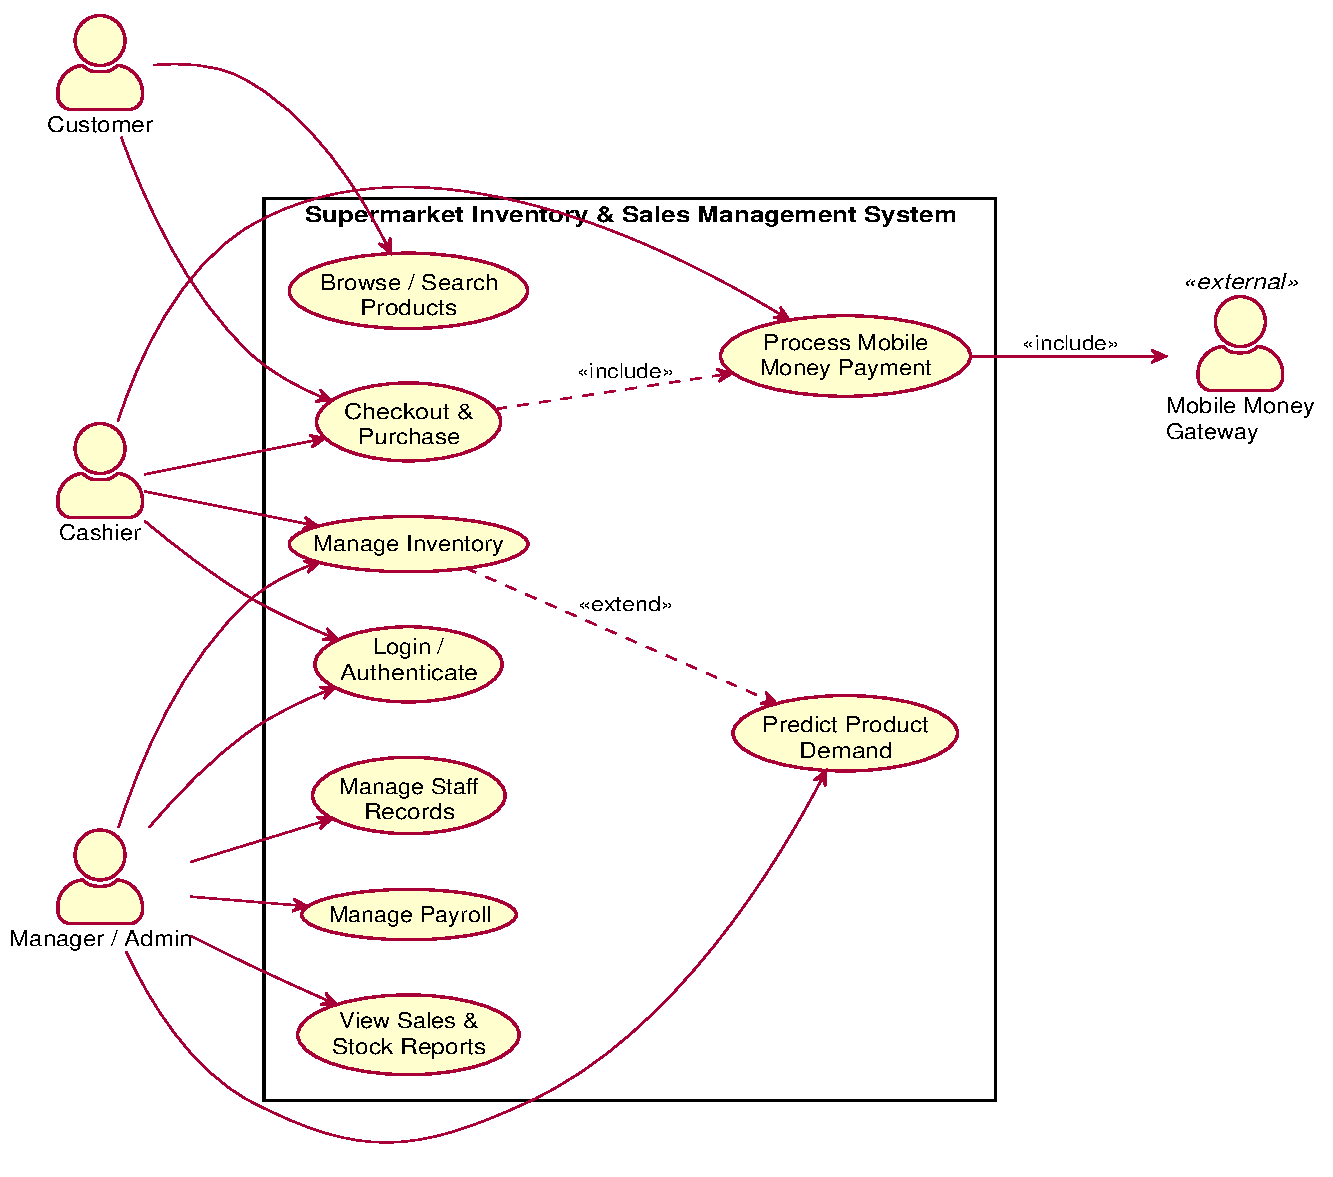
\includegraphics[width=\linewidth]{figures/01_usecase.pdf}
  \caption{Use case diagram for \sysname{}}
  \label{fig:usecase}
\end{figure}

\section{Actor Descriptions}
\begin{center}
\begin{tabular}{@{}p{3.3cm}p{10.4cm}@{}}
\toprule
\textbf{Actor} & \textbf{Description} \\
\midrule
Customer & Purchases products and pays via mobile money. \\
Cashier & Operates the point of sale, processes checkouts and payments. \\
Manager/Admin & Manages inventory, staff, payroll, demand forecasts and reports. \\
Mobile Money Gateway & External payment provider used for customer payments and staff payouts. \\
\bottomrule
\end{tabular}
\end{center}

\section{Key Use Case Specification: Process Mobile Money Payment}
\begin{center}
\begin{tabular}{@{}p{3.3cm}p{10.4cm}@{}}
\toprule
\textbf{Field} & \textbf{Description} \\
\midrule
Primary actor & Cashier (on behalf of Customer) \\
Preconditions & Sale total has been computed; customer has an active mobile money account \\
Main flow & (1) Cashier selects mobile money as payment method; (2) system sends a payment request to the gateway; (3) gateway prompts the customer for PIN confirmation; (4) customer confirms; (5) gateway returns approval; (6) system updates stock and prints a receipt \\
Alternate flow & If the gateway declines or times out, the cashier is prompted to retry or select another payment method \\
Postconditions & Sale is recorded, stock is decremented, payment is confirmed \\
\bottomrule
\end{tabular}
\end{center}

% ================= CHAPTER 4: STATIC STRUCTURE =================
\chapter{Static Structure -- Class Diagram}

\section{Overview}
Figure~\ref{fig:class} shows the core domain classes and their relationships, covering products and inventory, sales and payment, demand forecasting, and staff and payroll.

\begin{figure}[h!]
  \centering
  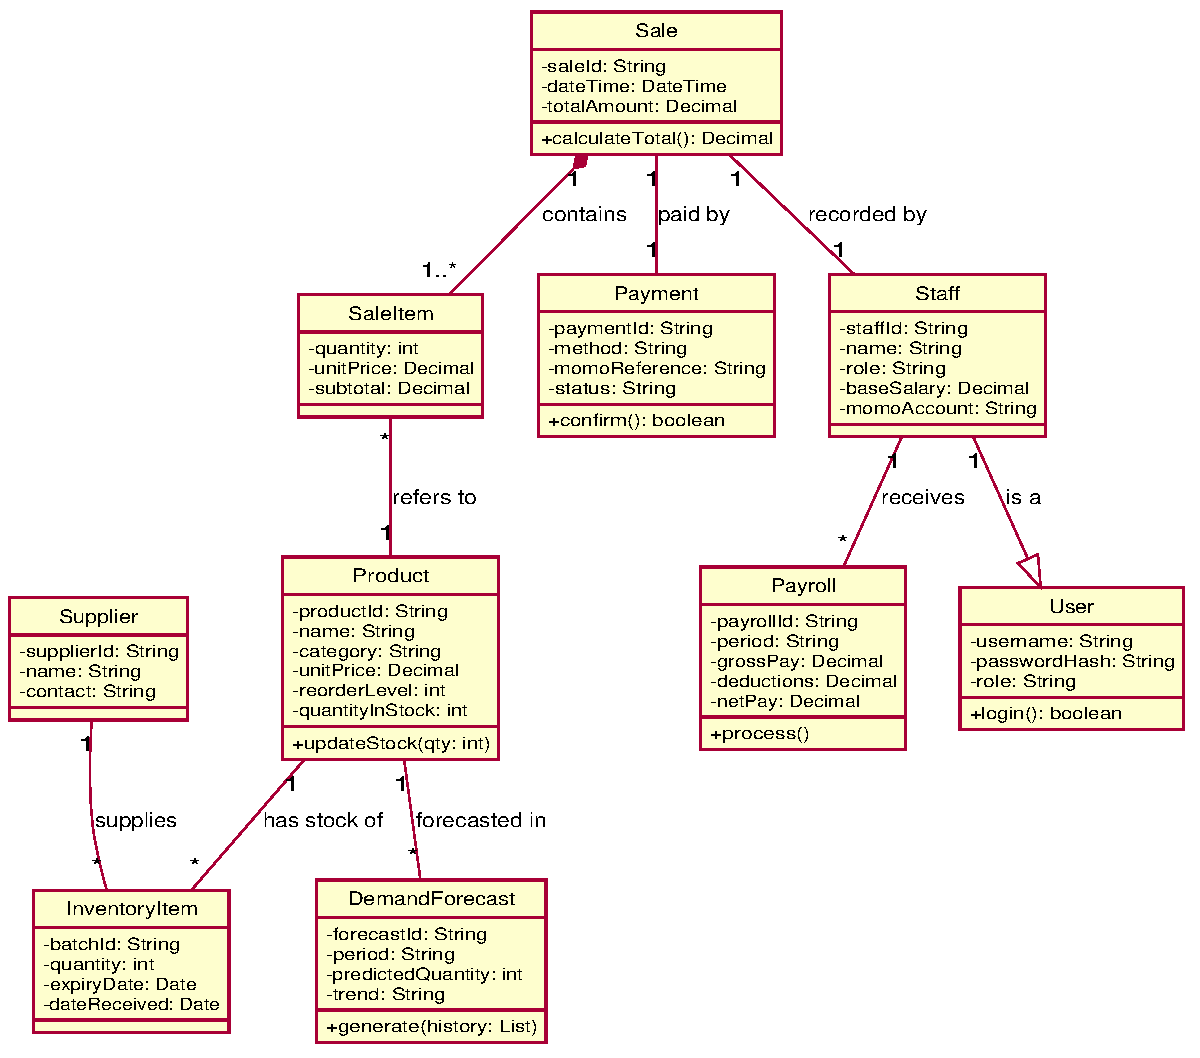
\includegraphics[width=\linewidth]{figures/02_class.pdf}
  \caption{Class diagram for \sysname{}}
  \label{fig:class}
\end{figure}

\section{Notable Design Decisions}
\begin{itemize}[leftmargin=1.4em]
  \item \texttt{DemandForecast} is linked to \texttt{Product} rather than embedded in it, keeping forecasting data versioned and separate from live stock counts.
  \item \texttt{Payment} is associated one-to-one with \texttt{Sale} and stores the mobile money reference (\texttt{momoReference}) returned by the gateway, so a transaction can be reconciled later.
  \item \texttt{Staff} generalizes from \texttt{User} to reuse authentication (login/role) across staff members without duplicating credential handling.
\end{itemize}

% ================= CHAPTER 5: DYNAMIC BEHAVIOUR =================
\chapter{Dynamic Behaviour}

\section{Sequence Diagram: Sale with Mobile Money Payment}
Figure~\ref{fig:seq1} traces a checkout from item scanning through mobile money confirmation and stock update.

\begin{figure}[h!]
  \centering
  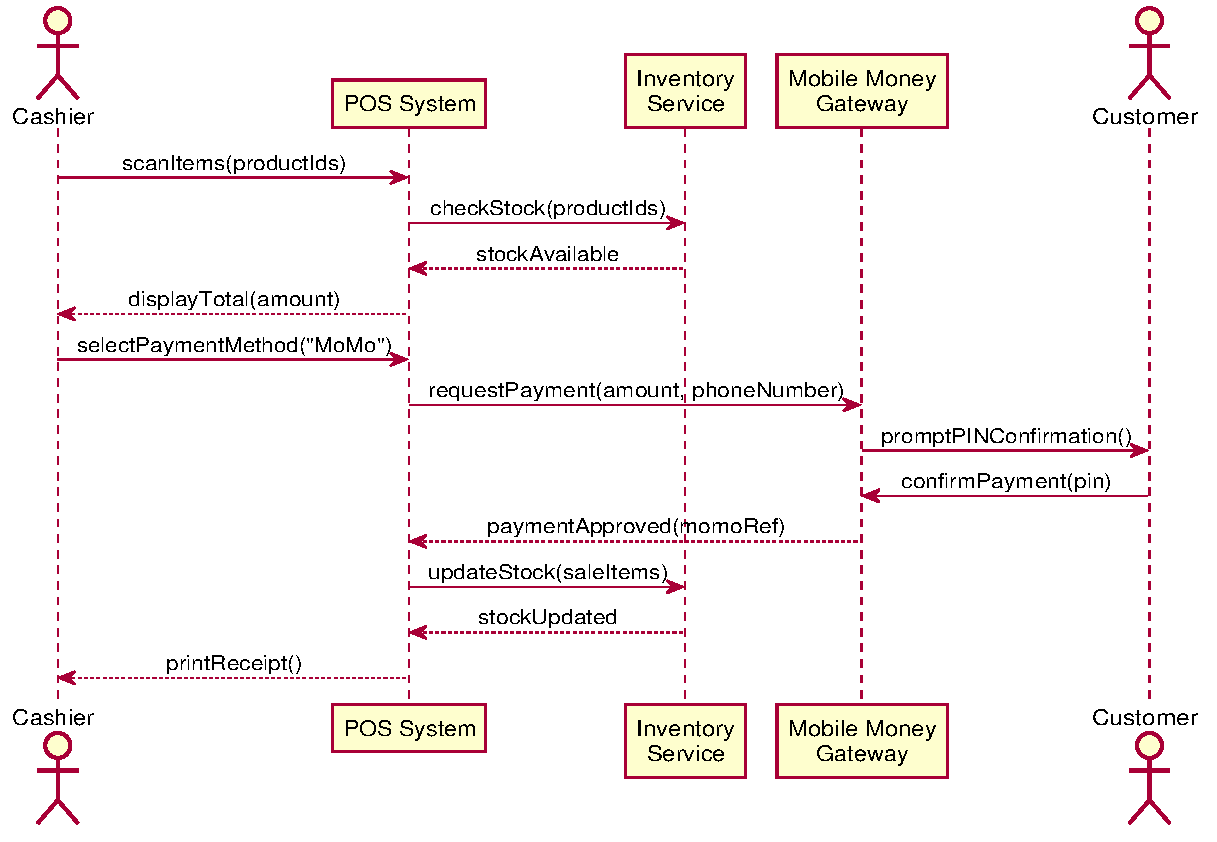
\includegraphics[width=\linewidth]{figures/03_seq_sale_payment.pdf}
  \caption{Sequence diagram: sale with mobile money payment}
  \label{fig:seq1}
\end{figure}

\section{Sequence Diagram: Demand Prediction Generation}
Figure~\ref{fig:seq2} shows how the system pulls historical sales data and passes it to the prediction engine to produce a forecast.

\begin{figure}[h!]
  \centering
  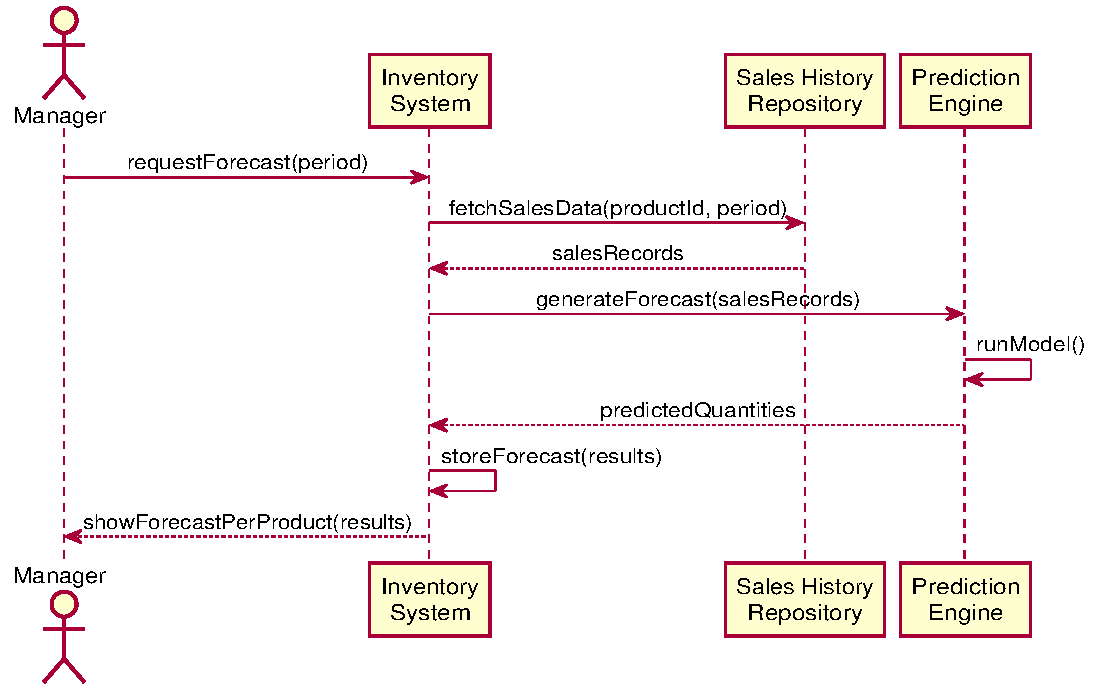
\includegraphics[width=\linewidth]{figures/04_seq_prediction.pdf}
  \caption{Sequence diagram: demand prediction generation}
  \label{fig:seq2}
\end{figure}

\section{Sequence Diagram: Staff Payroll Processing}
Figure~\ref{fig:seq3} shows payroll computation and mobile money payout to staff.

\begin{figure}[h!]
  \centering
  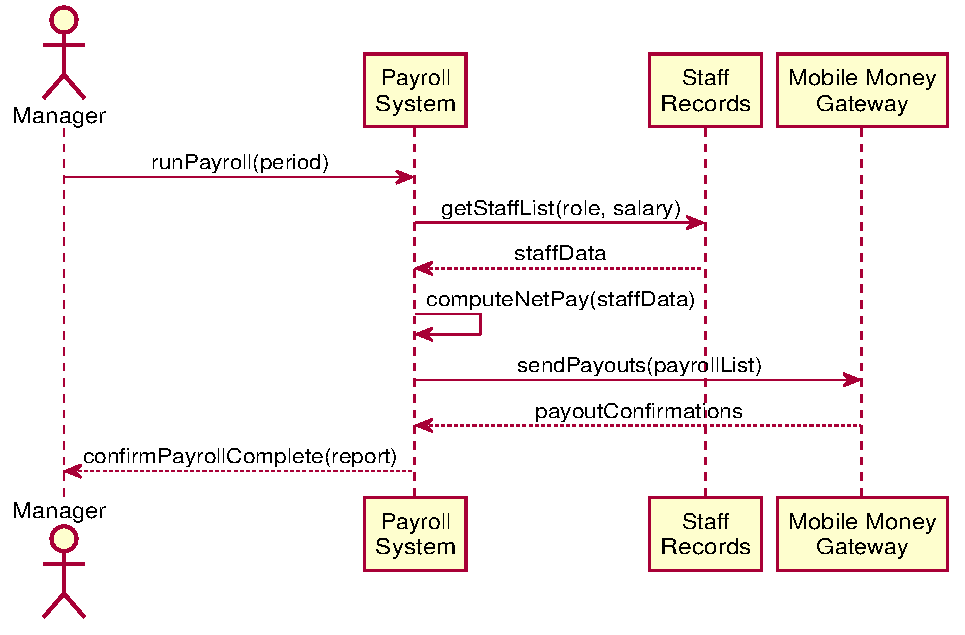
\includegraphics[width=\linewidth]{figures/05_seq_payroll.pdf}
  \caption{Sequence diagram: staff payroll processing}
  \label{fig:seq3}
\end{figure}

\section{Activity Diagram: Stock Replenishment}
Figure~\ref{fig:activity} shows the workflow triggered by the demand prediction: if predicted need exceeds current stock, a purchase order is raised, goods are received, and inventory is updated.

\begin{figure}[h!]
  \centering
  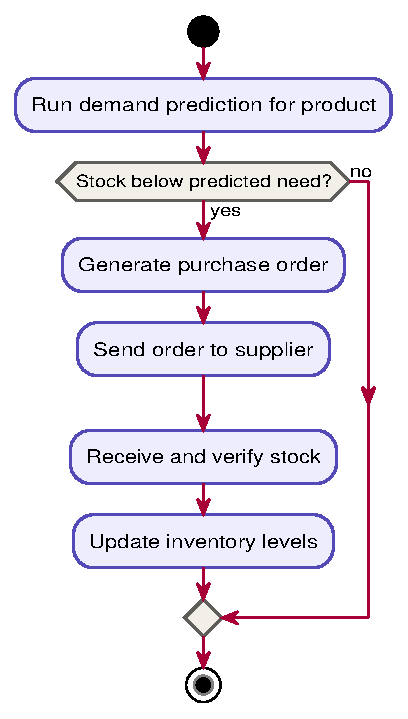
\includegraphics[width=0.65\linewidth]{figures/06_activity.pdf}
  \caption{Activity diagram: stock replenishment based on prediction}
  \label{fig:activity}
\end{figure}

\section{State Transition Diagram: Inventory Item}
Figure~\ref{fig:state} shows the lifecycle of an inventory item's stock status, from being fully stocked through low stock, out of stock, reorder, and back to in stock.

\begin{figure}[h!]
  \centering
  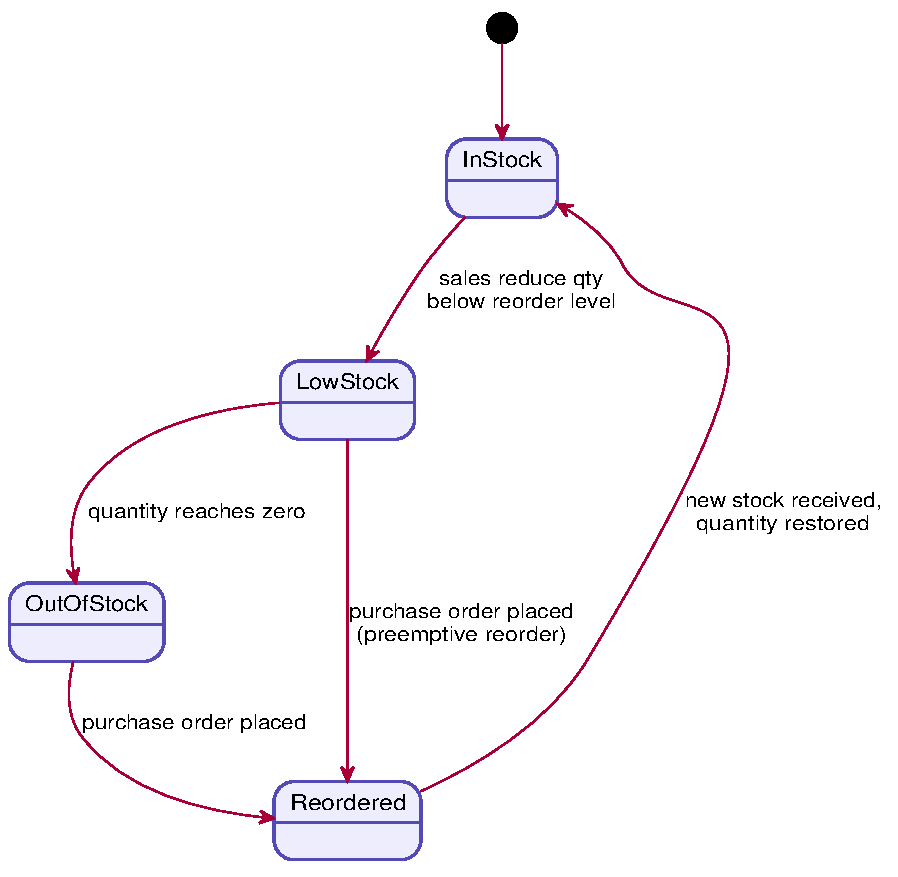
\includegraphics[width=\linewidth]{figures/07_state.pdf}
  \caption{State transition diagram: inventory item stock status}
  \label{fig:state}
\end{figure}

% ================= CHAPTER 6: NON-FUNCTIONAL =================
\chapter{Non-Functional Considerations}

\section{Reliability and Consistency}
Mobile money payment confirmation must be received before a sale is marked as paid; stock decrements only occur after payment approval to avoid inconsistent inventory state on payment failure.

\section{Scalability}
The prediction engine is designed as a separate logical component so that its computation (e.g. batch or scheduled forecasting runs) does not block point-of-sale transactions.

\section{Security}
Staff authentication reuses a common \texttt{User} credential model; mobile money references and payroll data are treated as sensitive and should be access-controlled to Manager/Admin roles.

\section{Auditability}
Every sale is linked to a payment record with a mobile money reference, and every payroll run produces a report, enabling reconciliation against the mobile money provider's statements.

\end{document}
